%
% LAYOUT.TEX - Kurzbeschreibung von PA 88-10-04 (LaTeX)
%                                      99-03-20
%
%  Updated for REFMAN.CLS (LaTeX2e)
%
\documentclass[twoside,a4paper]{refart}
%\documentclass[pagesize,twoside,a5paper,smallborder,10pt]{refart}
\usepackage[T1]{fontenc}
%\usepackage{ae} % CM-Zeichens"atze mit T1 encoding
\usepackage{makeidx}
\usepackage[colorlinks=true]{hyperref}
\usepackage[per-mode=symbol]{siunitx}
\DeclareSIUnit \dBm {dBm}
\usepackage{tcolorbox}

\usepackage{graphicx}
\usepackage{float}

\usepackage[iso,english]{isodate}
\usepackage[labelformat=simple]{subcaption}

\DeclareRobustCommand\cs[1]{\texttt{\char`\\#1}}

% BOARD-REVISION string will be replaced by the CI script with the latest
% board revision number taken from the KiCad PCB files.
% Do not change the BOARD-REVISION string!
\title{RedPitaya Lockbox -- Manual\\
	\textit{\normalsize{Latest board revision BOARD-REVISION}}}
\author{Patrick Baus, Tilman Preuschoff, Tobias Schreiber}

\date{Last modified: \today}
\emergencystretch1em  % F"ur TeX <3.0 auskommentieren!


\makeindex


\setcounter{tocdepth}{2}
\settextfraction{0.7}

\begin{document}
\maketitle
\begin{maxipage}
	\centering
	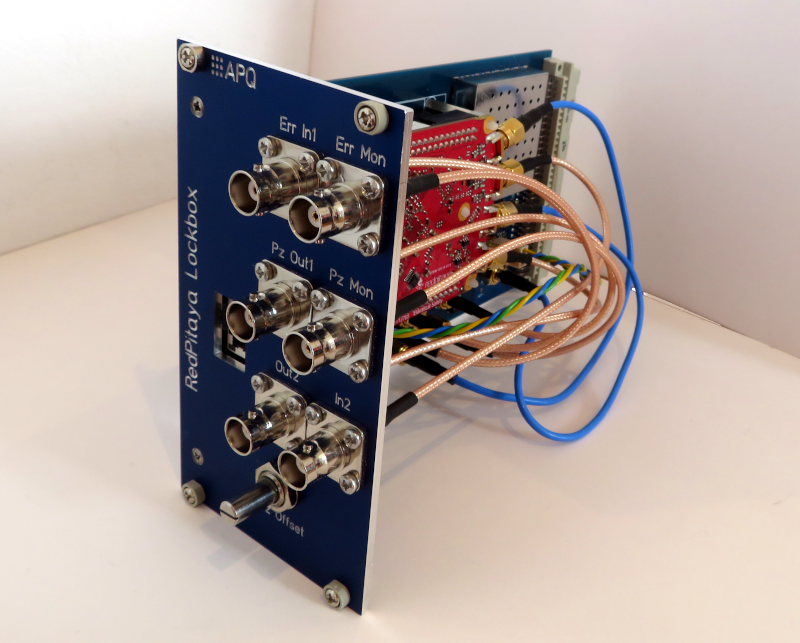
\includegraphics[width=0.9\textwidth]{fig/lockbox.png}
\end{maxipage}
\begin{abstract}
	The \href{https://github.com/TU-Darmstadt-APQ/RedPitaya-Lockbox}{RedPitaya lockbox} is a fast digital controller for laser frequency stabilization. The commercial FPGA based \href{https://www.redpitaya.com/f130/STEMlab-board}{RedPitaya STEMlab 125-14} board is complemented by an analog interface that provides all necessary functionalities -- such as an error signal input stage, two control loops for laser current and piezo including a piezo driver and additonal monitoring outputs. The device is operated with the open-source software package \href{https://pyrpl.readthedocs.io/en/latest/}{PyRPL}.  
\end{abstract}
\newpage

\tableofcontents

%%%%%%%%%%%%%%%%%%%%%%%%%%%%%%%%%%%%%%%%%%%%%%%%%%%%%%%%%%%%%%%%%%%%


\section{Setting up the RedPitaya}

\subsection{Mounting the RedPitaya on the lockbox PCB}

\index{RedPitaya OS}\marginlabel{Install the RedPitaya OS} Install the RedPitaya OS on a microSD card (4 GB min.) following the instructions on \href{https://redpitaya.readthedocs.io/en/latest/quickStart/SDcard/SDcard.html}{https://redpitaya.readthedocs.io/en/latest/quickStart/ SDcard/SDcard.html}. PyRPL has been tested with software release 0.94 to 0.99. Use the latest release if possible. Older releases can be found here: \href{http://downloads.redpitaya.com/downloads/}{http://downloads.redpitaya.com/ downloads/}. A local copy of the latest image can be found on $\backslash$$\backslash$brain42$\backslash$public$\backslash$Labortechnik $\backslash$Elektronik$\backslash$RedPitay$\backslash$Images. Insert the card in the SD slot of the RedPitaya after installation.

\index{Offset resistors}\marginlabel{Remove the DC-offsets}
Remove the noisy DC-offset for both fast RedPitaya outputs by removing the four resistors marked in Fig.~\ref{fig:offset}. Use a standard soldering iron. This shifts the output voltage range from $\pm$\qty{1}{\volt} to \qty{0}{\volt}--\qty{2}{\volt}. Additional information can be found on \href{https://ln1985blog.wordpress.com/2016/02/07/red-pitaya-dac-performance/}{https://ln1985blog.wordpress.com/ 2016/02/07/red-pitaya-dac-performance/}. After removing the resistors, label the board accordingly (e.g. 'offset removed').

\textbf{Note:} The software (PyRPL and STEMlab) will still display and assume a $\pm$\qty{1}{\volt} range.

\textbf{Note:} The default output is now \qty{1}{\volt} instead of \qty{0}{\volt}.

\textbf{Note:} The RedPitaya output cannot drive a \qty{50}{\ohm}-load at \qty{2}{\volt}. Use a high-Z buffer (also in order to avoid cross talk between the two outputs).
\textbf{Edit:} In PCB Rev 1.4 a sufficient output buffer was added. 

\begin{figure}[H]
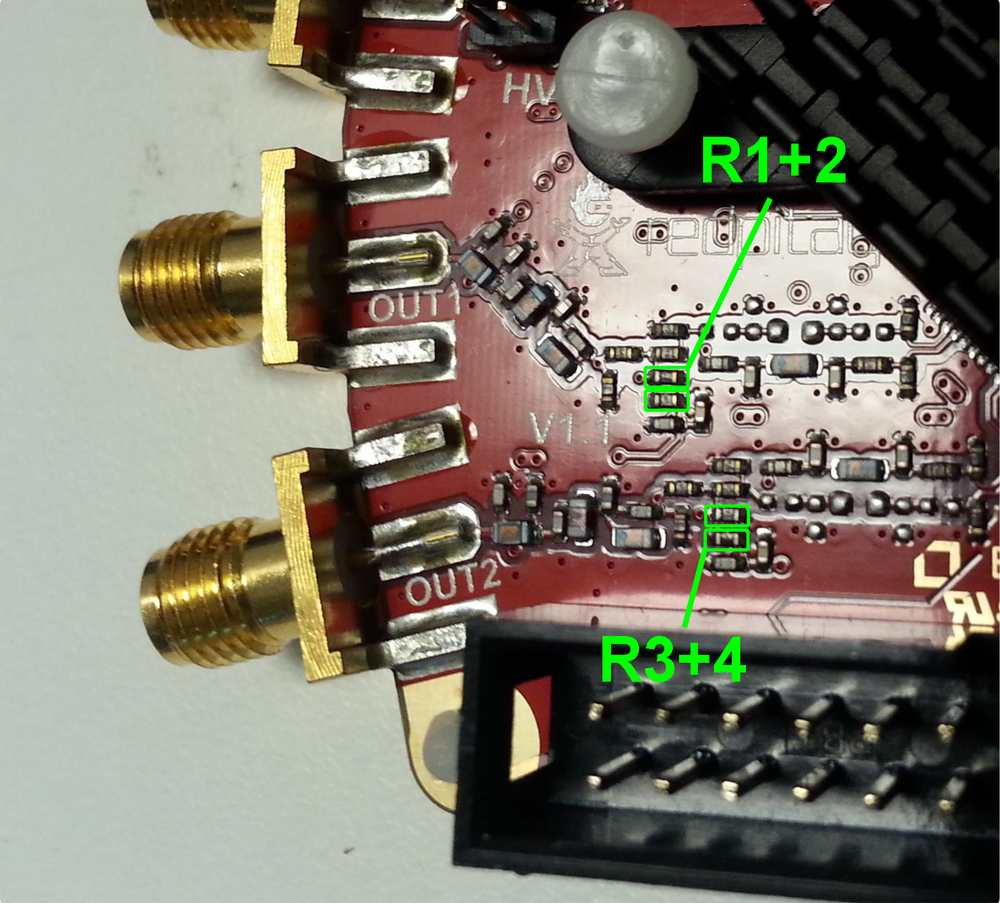
\includegraphics[width=\textwidth]{fig/offset-removal.png}
\caption{RedPitaya fast output offset resistors. [Image by L. Neuhaus]\label{fig:offset}}
\end{figure}

\index{Mount the RedPitaya}\marginlabel{Mount the RedPitaya board on the PCB}
Move the four nylon PCB mounts of the RedPitaya to the other side of the board. Attach \qty{17}{\milli\meter} hexnut M3 distance bolts to the PCB mounts using headless M3-screws. Connect the RedPitaya board (upside down) to the 26-pin IDC-connector on the PCB. Fix the board using M3 pan head screws and M3 washers.

\textbf{Note:} The RedPitaya's MAC address is denoted on the network connector. Make sure to remember it since it will not be visible after mounting the board. 

\textbf{Note:} Make sure all inputs are set to the low voltage range 'LV' (Fig.~\ref{fig:jumper}). See also \href{https://redpitaya.readthedocs.io/en/latest/developerGuide/125-14/fastIO.html#analog-inputs}{https://redpitaya.readthedocs.io/en/latest/developer Guide/125-14/fastIO.html\#analog-inputs}.

\begin{figure}[H]
	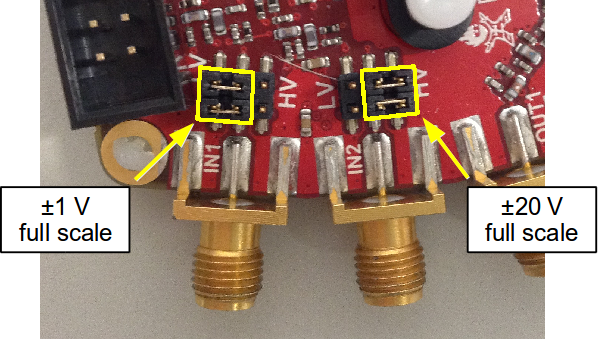
\includegraphics[width=\textwidth]{fig/Jumper_settings_photo.png}
	\caption{Jumper settings for $\pm$\qty{1}{\volt} and $\pm$\qty{20}{\volt} input range.\label{fig:jumper}}
\end{figure}


\begin{figure}[H]
	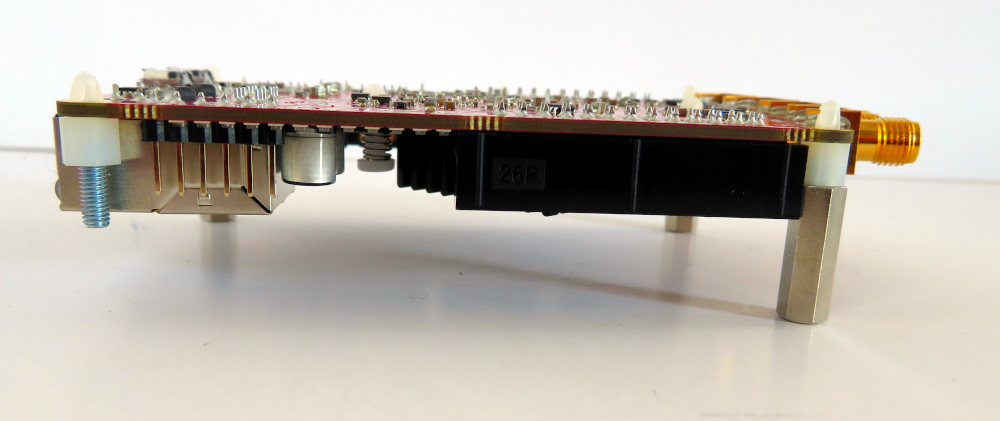
\includegraphics[width=\textwidth]{fig/mounting.png}
	\caption{RedPitaya board PCB mounting assembly.\label{fig:mounting}}
\end{figure}
\begin{figure}[H]
	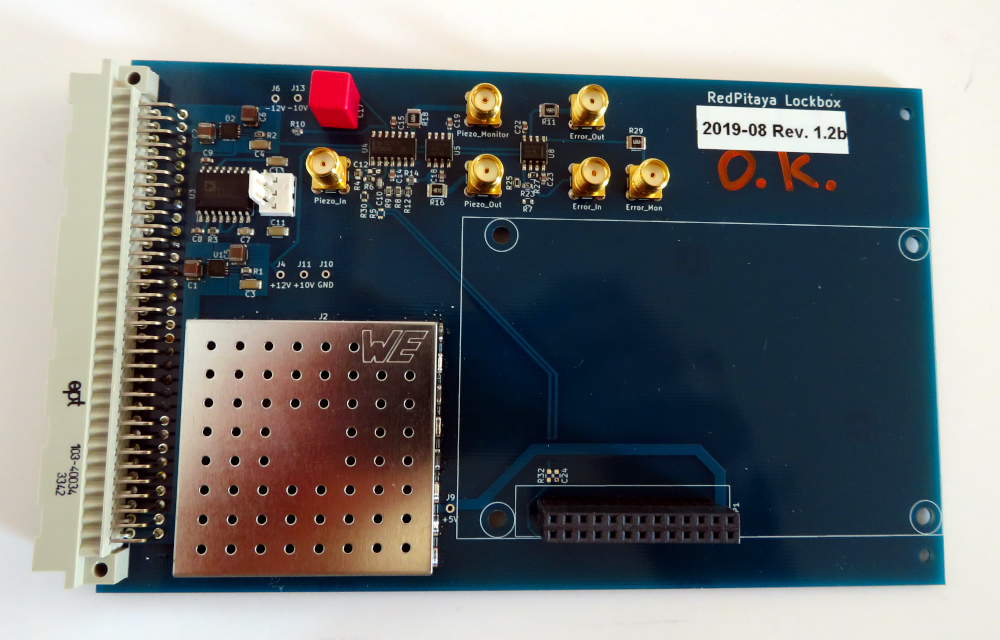
\includegraphics[width=\textwidth]{fig/PCB_lockbox.png}
	\caption{Fully assembled RedPitaya Lockbox PCB (Rev1.2b).\label{fig:PCB}}
\end{figure}
\begin{figure}[H]
	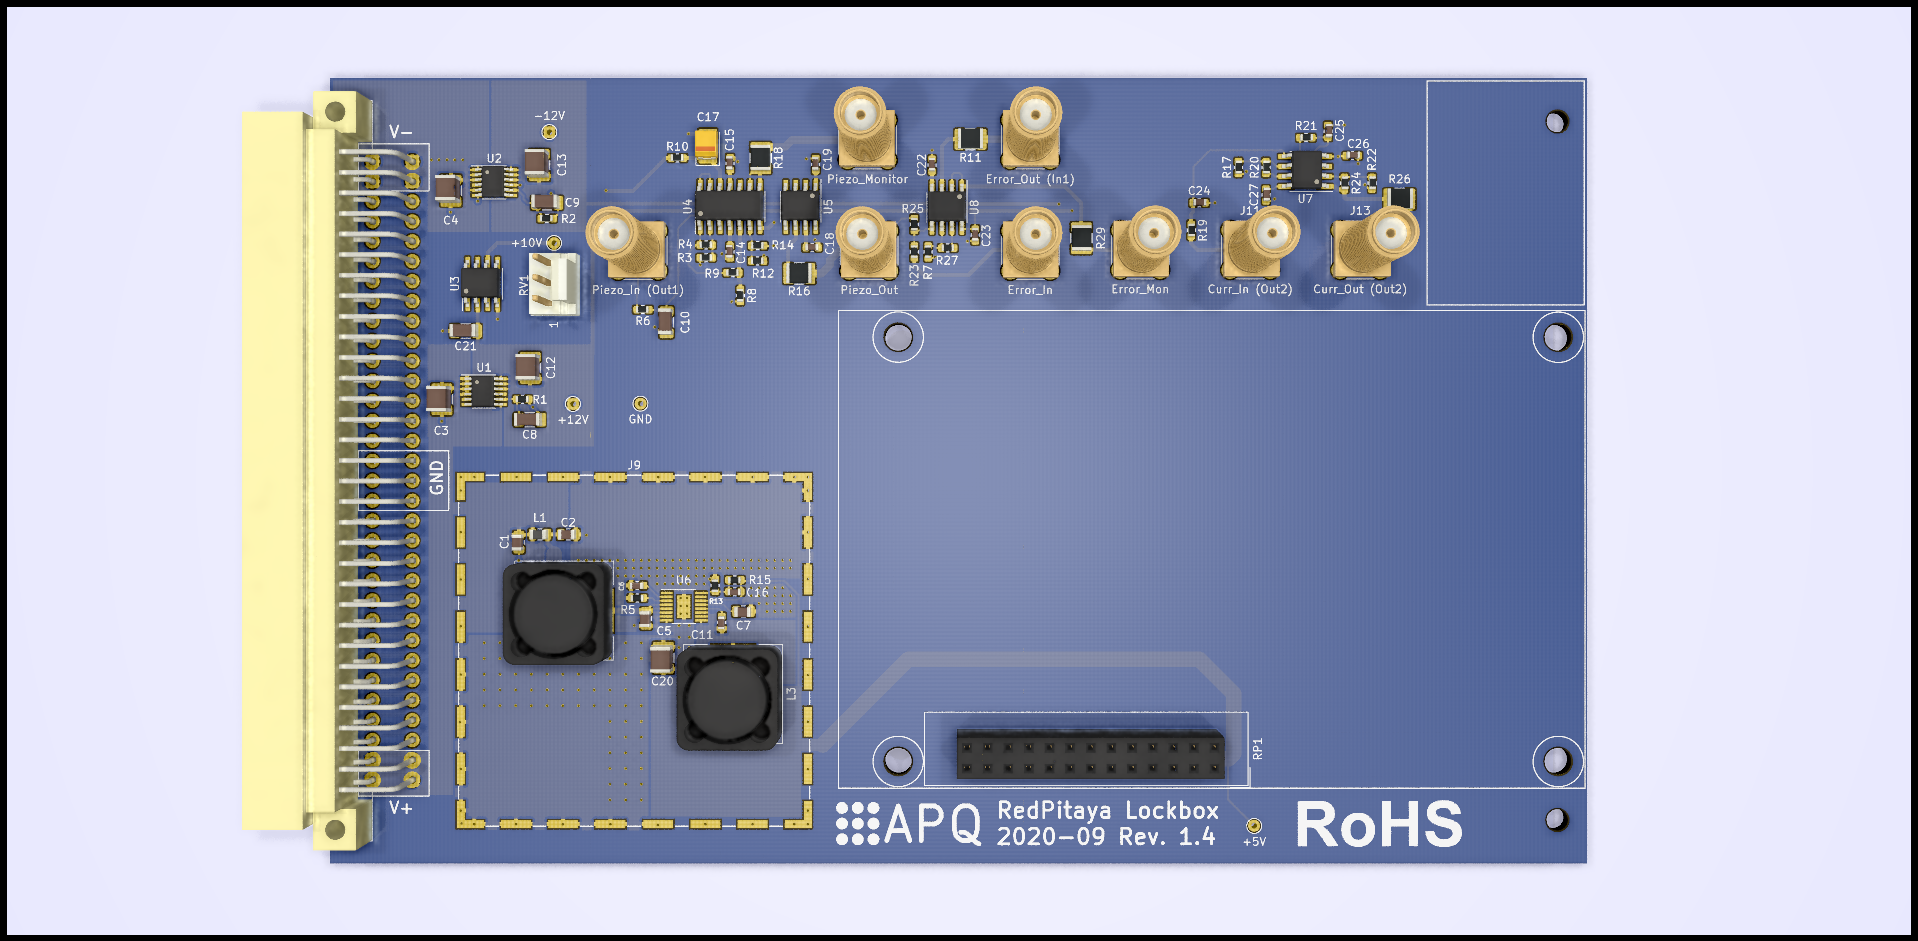
\includegraphics[width=\textwidth]{fig/RedPitaya_Lockbox.png}
	\caption{3D-model of the latest PCB revision 1.4.\label{fig:PCB_3D}}
\end{figure}

\index{Front panel}\marginlabel{Install the front panel}
Use a pre assembled front panel and three additional \qty{20}{\centi\meter} SMA cables. Fix the front panel on the lockbox PCB using two \qty{10}{\milli\meter} pan head M2.5 screws and M2.5 washers. Connect the cable according the table below.

\begin{tabular}{|c|c|c|}\hline
\textbf{Front panel} & \textbf{PCB} 			& \textbf{RedPitaya}	\\\hline
ErrIn1		& Error\_In		& 	 		\\\hline	
ErrMon		& Error\_Mon	&			\\\hline
PzOut1		& Piezo\_Out	&			\\\hline
PzMon		& Piezo\_Monitor&			\\\hline
Out2		& Curr\_Out		& 			\\\hline
In2			&				& In2		\\\hline
PzOffset	& RV1			&			\\\hline
			& Error\_Out	& In1		\\\hline
			& Piezo\_In		& Out1		\\\hline
			& Curr\_In		& Out2		\\\hline
\end{tabular}

\textbf{Note:} In PCB Rev 1.4 an output buffer and filter for 'Out2'  (current) was added. For PCB revisions earlier than 1.4 connect the RedPitaya's output2 directly to the front panel (Out2).

\begin{figure}[H]
	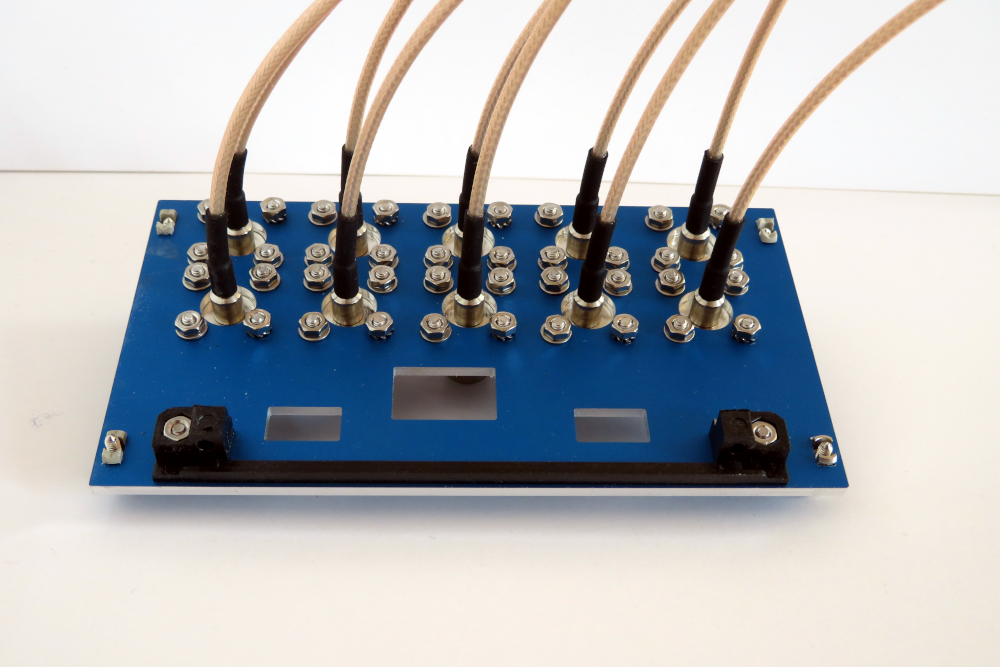
\includegraphics[width=\textwidth]{fig/front_panel.png}
	\caption{Pre-assembled front panel (RedPitaya IntStab).\label{fig:front_panel}}
\end{figure}

\index{Potentiometer}\marginlabel{Installing the potentiometer}
The front panel requires a \num{10}-turn potentiometer. This needs to be correctly wired to a \href{Molex KK 254}{} connector on the PCB using three twisted stranded wires. The colour ode of these wires is
\begin{itemize}
	\item Black (GND, clockwise/CW)
	\item Green (wiper/slider/S)
	\item Yellow (reference, counterclockwise/CCW)
\end{itemize}

Do note, that the pin number on the Vishay 534 does not match the pin numbering given in the schematics. Use the CW and CCW  labels for orientation. This ensures that when turning the potentiometer clockwise an increasing voltage is added to the piezo output. Figure \ref{fig:potentiometer_example} shows two example pictures for both the Vishay 534 and its alternative, the Bourns 7276 potentiometer. Also shown is the Molex KK connector with the correct colour coding. Before soldering the wires to the potentiometer make sure you add shrink tubing as shown in figure \ref{fig:potentiometer_example_vishay}.

\begin{figure}[H]
	\begin{subfigure}{0.45\textwidth}
		\centering
		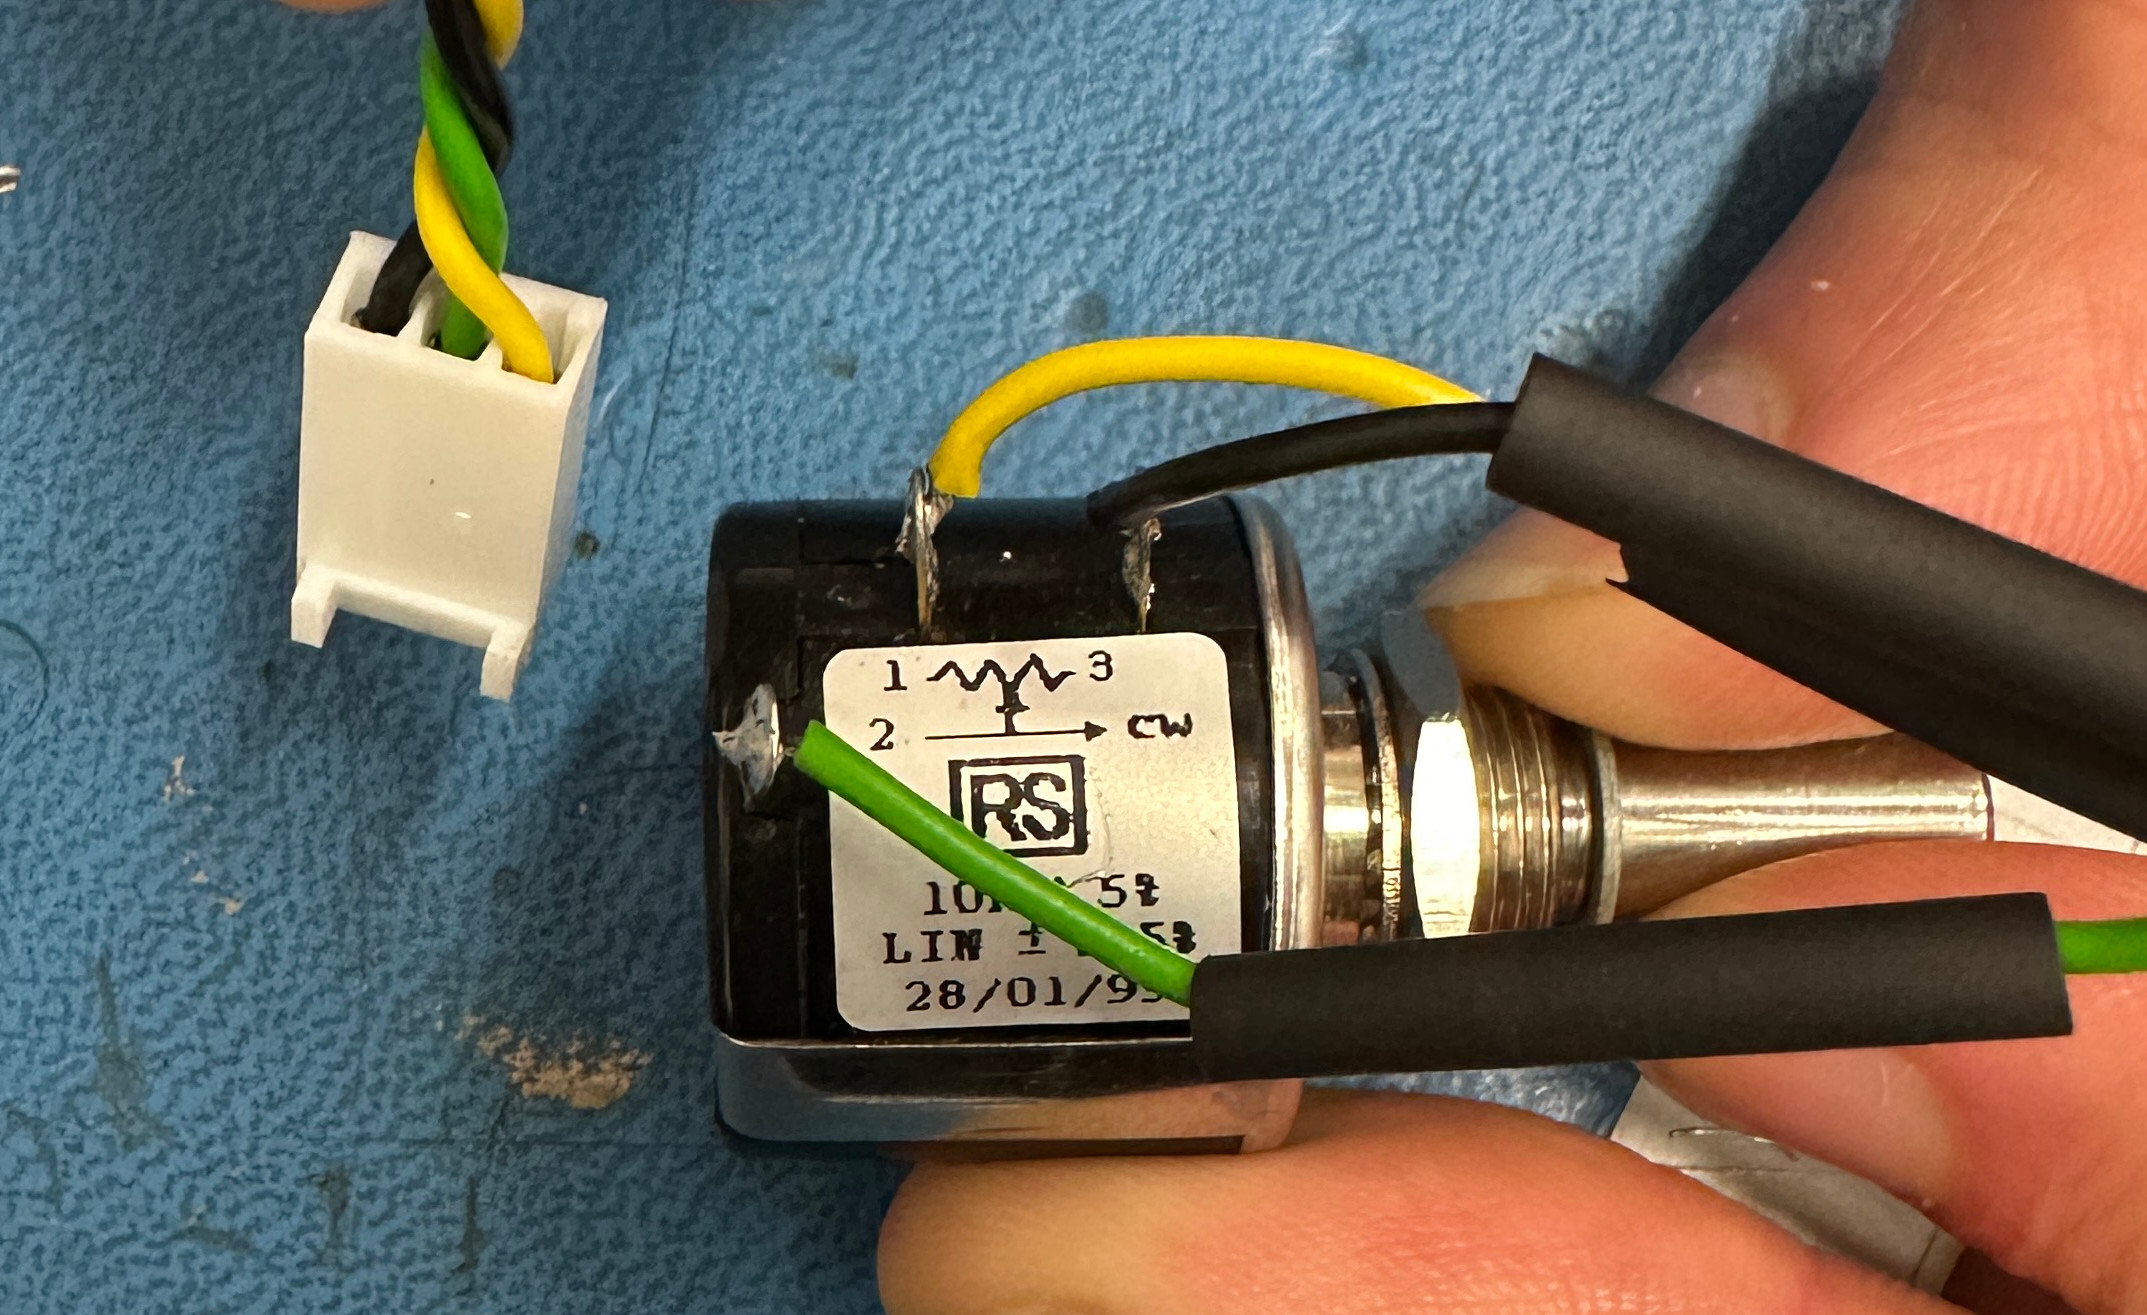
\includegraphics[width=\linewidth]{fig/potentiometer_vishay.jpg}
		\caption{Vishay 534}
		\label{fig:potentiometer_example_vishay}
	\end{subfigure}
	\begin{subfigure}{0.45\textwidth}
		\centering
		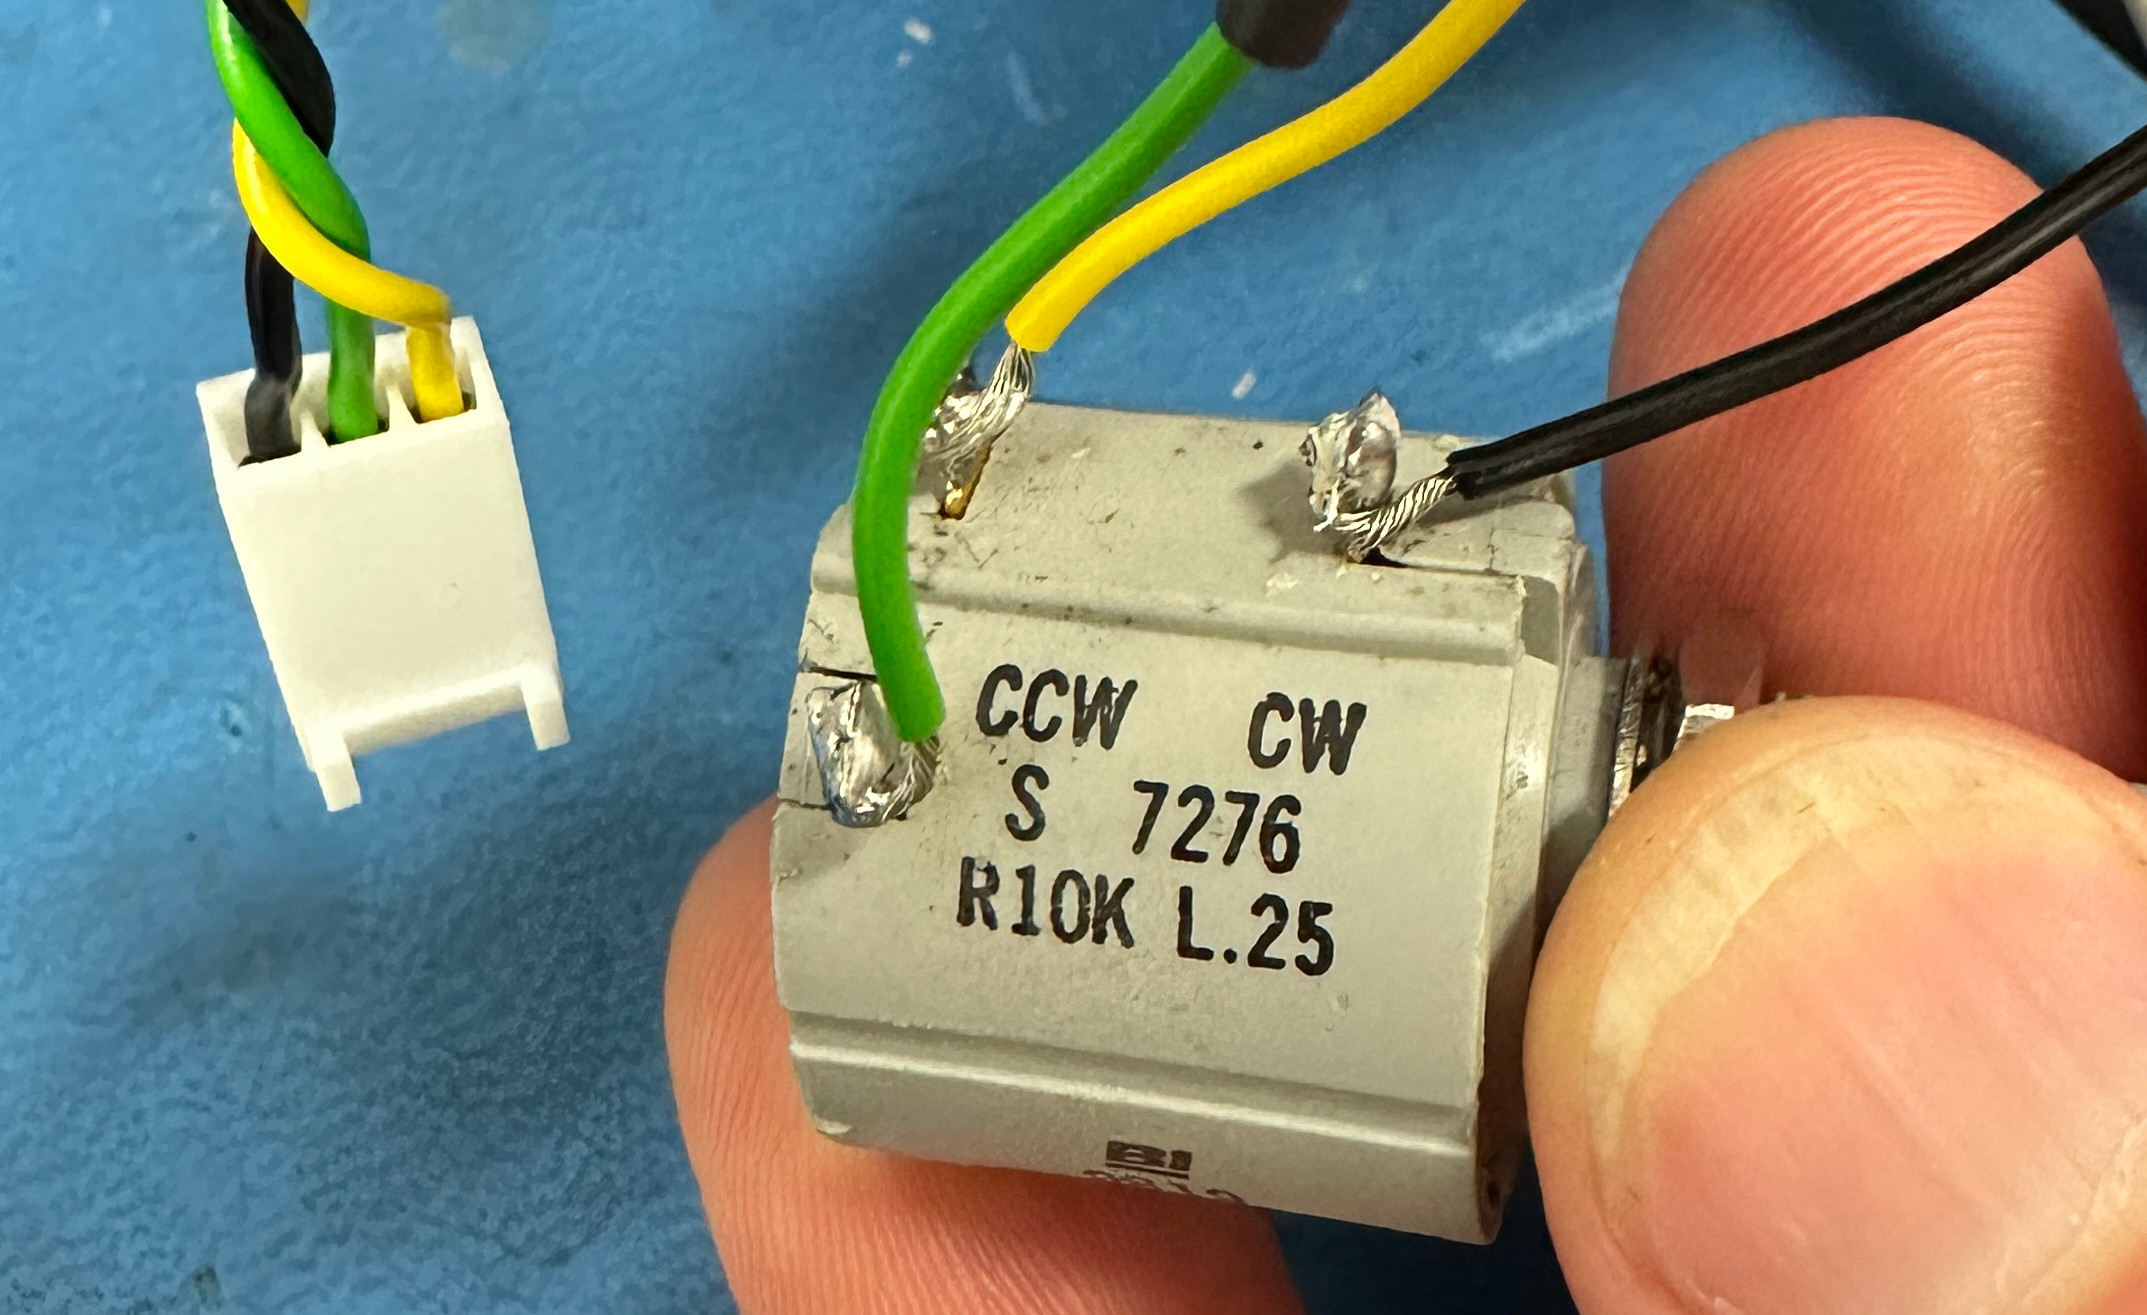
\includegraphics[width=\linewidth]{fig/potentiometer_bourns.jpg}
		\caption{Bourns 7276}
	\end{subfigure}
	\caption{Example wiring for different potentiometers.}
	\label{fig:potentiometer_example}
\end{figure}

Once the wires are soldered and before shrinking the shrink tubing, the result should look like shown in figure \ref{fig:potentiometer_assemby}. Do note the twisted stranded wires as well.

\begin{figure}[H]
	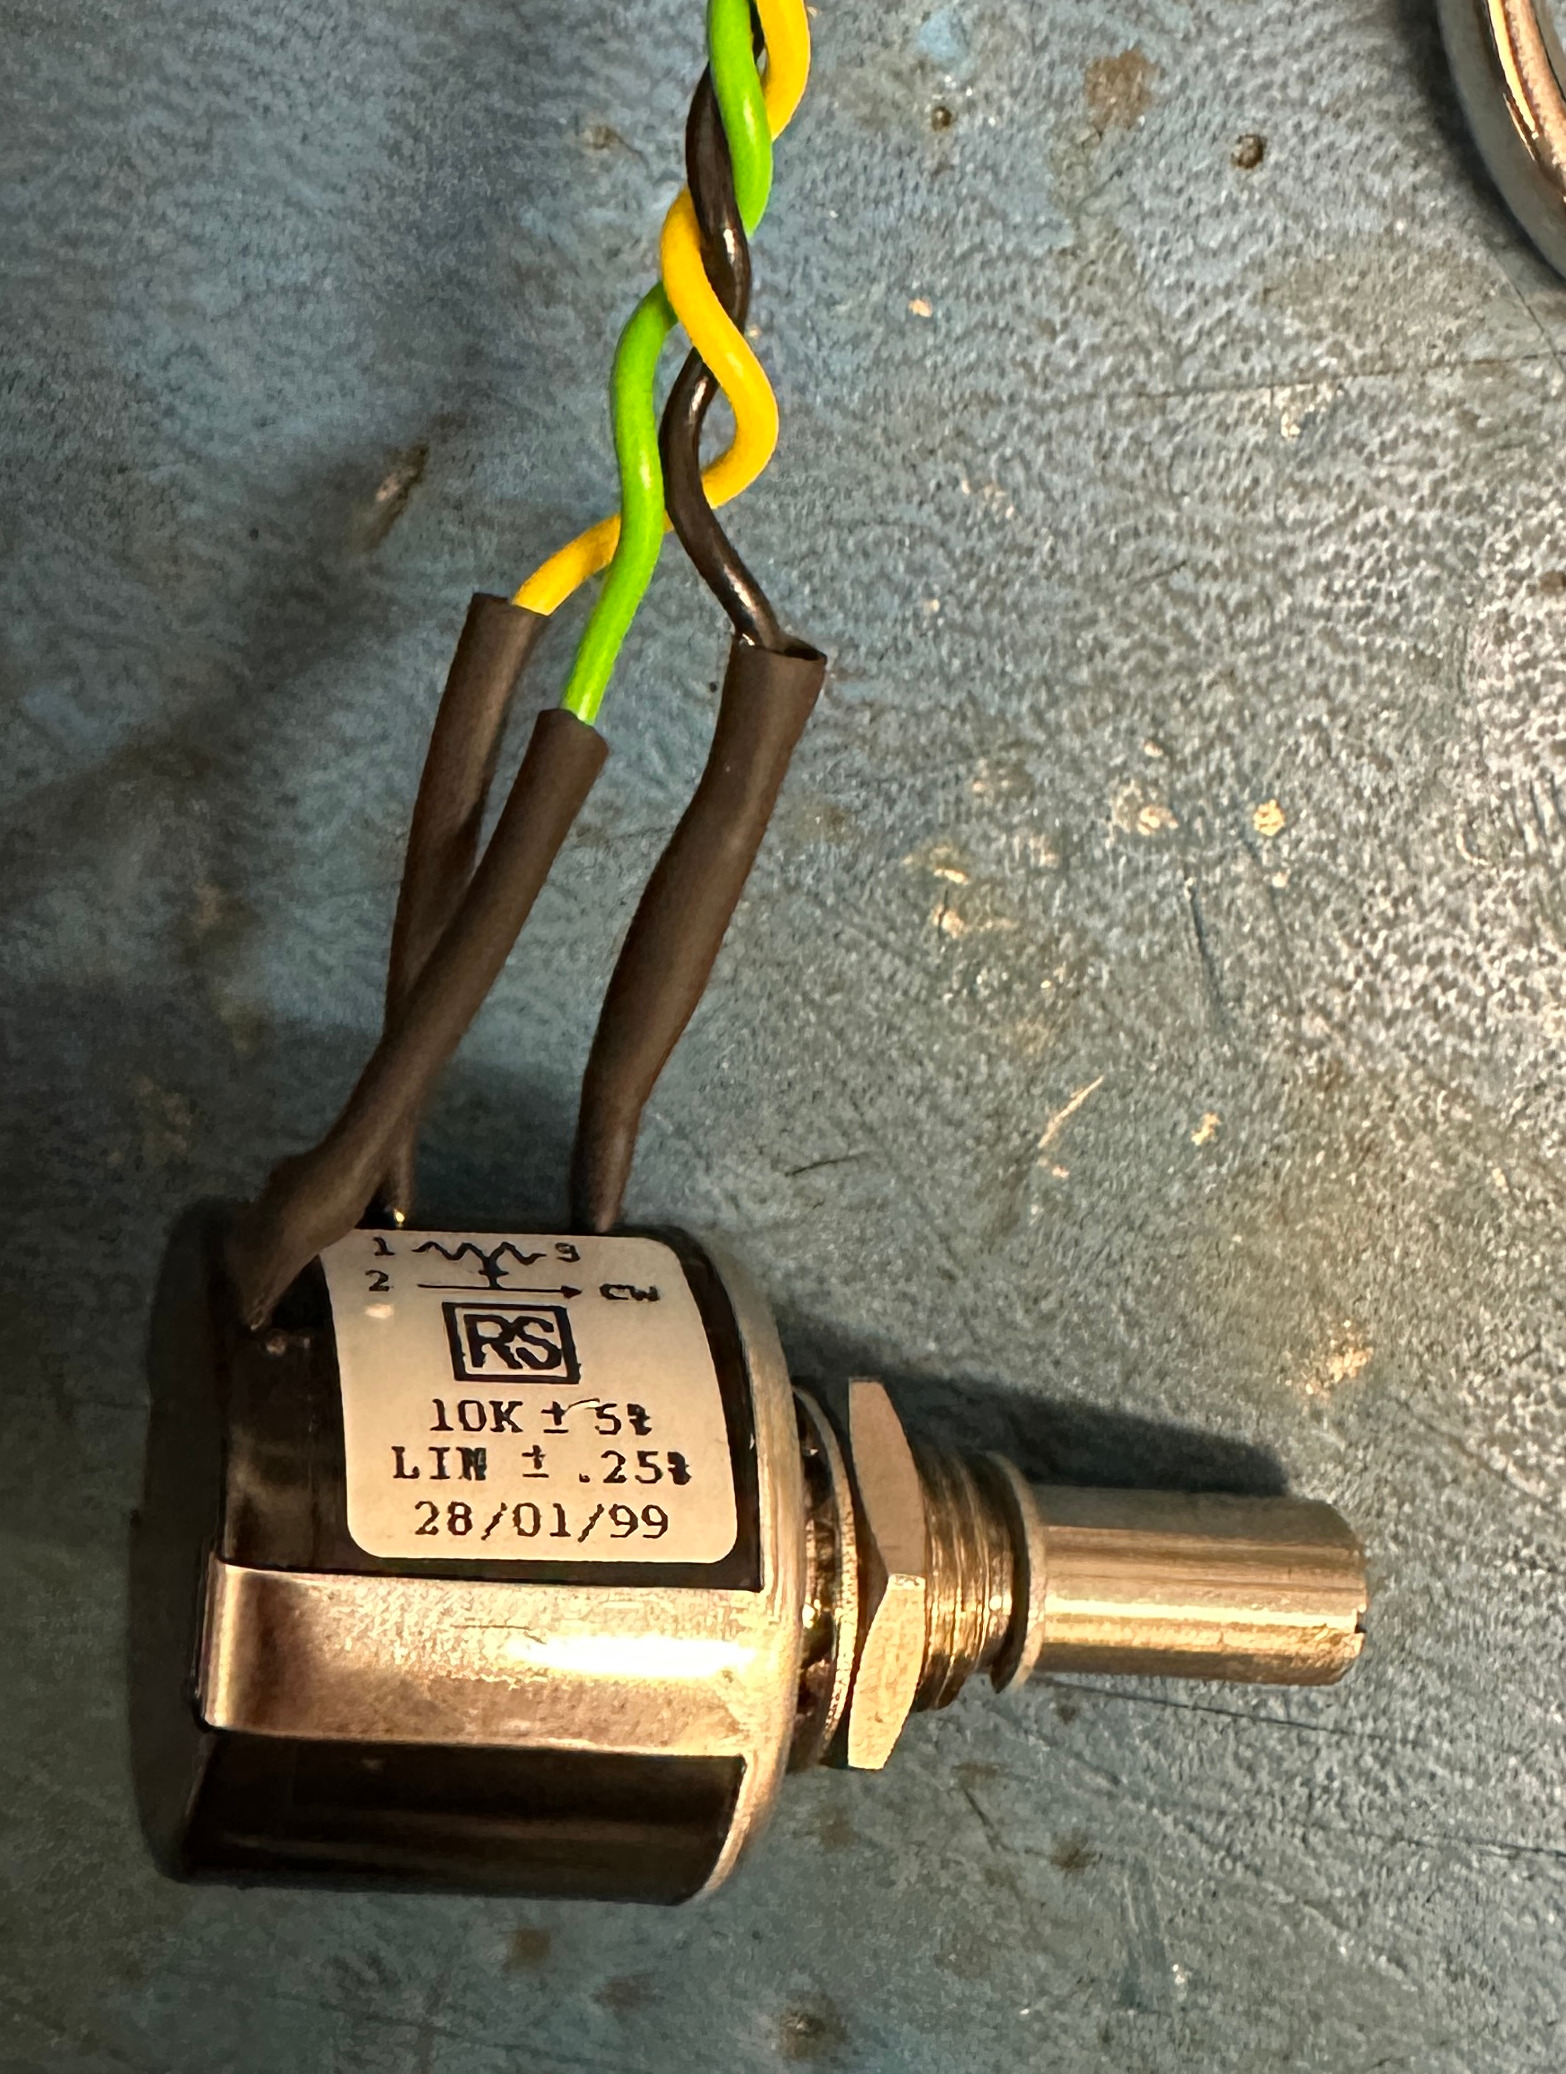
\includegraphics[width=0.5\textwidth]{fig/potentiometer_finished.jpg}
	\caption{Fully assembled potentiometer.}
	\label{fig:potentiometer_assemby}
\end{figure}


\subsection{Power supply and network connection}
\index{Power supply}\marginlabel{Power supply}
The RedPitaya lockbox is mounted in a 19-inch Fischer rack mount unit with our standard power supply (DIN41612 C64A/C connector). A \qty{\pm 15}{\volt} supply is recommended.

\begin{maxipage}
	\centering
\begin{table}[H]
	{\small
		\begin{tabular}{|c|c|c|c|}\hline
			\textbf{Supply} & \textbf{Voltage range} & \textbf{Current@15\,V (typ./max.)}	& \textbf{Pin config. (default / Toptica)}  \\\hline
			V+			& \qtyrange{12.5}{20}{\V}		& 	 \qty{0.35}{\A} / \qty{1.00}{\A}					& 1A, 1C, 2A, 2C	/  31A, 31C	 \\\hline
			V-			& \qtyrange{-20}{-12.5}{\V} 	&		\qty{0.05}{\A} / \qty{0.15}{\A}					& 31A, 31C, 32A 32C	/ 30A, 30C\\\hline
			GND			& -					&	-										& 16A, 16C, 17A, 17C, 18A, 18C  /  1A, 1C              \\\hline
		\end{tabular}
	}
	\caption{RedPitaya lockbox power supply rating. For connector pin configuration, see \href{https://b2b.harting.com/files/download/PRD/PDF_TS/0903164X921_100072506DRW176A.pdf}{Harting 09031646921}. \label{tab:power}}
\end{table}
\end{maxipage}

\textbf{Note:} Always check the power supply polarity and current rating before connecting the lockbox. Permanent damage to the device may occur by reverse polarity. The RedPitaya requires a larger current while powering up.

\index{Network connection}\marginlabel{Network connection:} Connect the RedPitaya to the local network. The color code for RedPitaya network cables is blue. Per default the RedPitaya IP address is acquired via DHCP (see also next section). 


\section{Setting up the software}

\index{PyRPL}\marginlabel{Install PyRPL} 
The RedPitaya is operated with the Python software package PyRPL. You need a proper Python installation in order to run the software. For Windows OS, use \href{https://www.anaconda.com/}{Anaconda Python}. Create a virtual environment for PyRPL. Get \textit{pyrpl-env.yaml} from \href{https://github.com/TU-Darmstadt-APQ/RedPitaya-Lockbox/tree/master/pyrpl}{https://github.com/TU-Darmstadt-APQ/RedPitaya-Lockbox/tree/master/pyrpl} and run (in the directory of the file)

\begin{tcolorbox}
	\begin{verbatim}
		conda env create -f pyrpl-env.yaml
	\end{verbatim}
\end{tcolorbox}

\textbf{Note:}  PyRPL is not compatible with the latest python and numpy version.

Activate the environment via

\begin{tcolorbox}
	\begin{verbatim}
		conda activate pyrpl-env
	\end{verbatim}
\end{tcolorbox}

Clone or download the branch 'external\_pid\_pause' from \href{https://github.com/lneuhaus/pyrpl/tree/external_pid_pause}{https://github.com/ lneuhaus/pyrpl/tree/external\_pid\_pause}. In the directory of the source files, run:

\begin{tcolorbox}
	\begin{verbatim}
	python setup.py develop
	\end{verbatim}
\end{tcolorbox}

\textbf{Note:} The branch 'external\_pid\_pause' is not the latest stable version of PyRPL. It will not be updated. If the installation does not work correctly and the sample and hold feature is not used, try installing the 'master' branch in a new environment.

\textbf{Known issues:}
\begin{itemize}
	\item 'pid'-module: Output limits seem to have a \qty{-1}{\volt} offset resulting in a max. output of \qty{0}{\volt}. Applying a \qty{1}{\volt} DC-offset with the 'asg'-module fixes the problem.
	\item 'lockbox' module: 'sweep' is only activated when the 'pid'-module is active.
\end{itemize}   

\index{IP and network}\marginlabel{Check the network connection and find the IP:}
The STEMlab web interface can be used for that task. Open this URL with a computer in the RedPitaya's local network:
\begin{tcolorbox}
	\begin{verbatim}
	http://rp-******.local
	\end{verbatim}
\end{tcolorbox}
Replace ****** by the last six digits of the RedPitaya's MAC address. Navigate to Settings$\rightarrow$Network in order to find the IP.

\textbf{Note:}
Label the front panel with the device IP, MAC-address and PCB revision.


\index{password}\marginlabel{Set the RedPitaya password} The default login for SSH connection to the RedPitaya is

\begin{tcolorbox}
	\begin{verbatim}
	User: root    Password: root
	\end{verbatim}
\end{tcolorbox}

Connect to the RedPitaya using a SSH terminal (e.g. \href{https://www.putty.org/}{putty}). The password can be changed with the command:
\begin{tcolorbox}
	\begin{verbatim}
	passwd
	\end{verbatim}
\end{tcolorbox}

\textbf{Note: }The password will be saved in plain text in the PyRPL config.-file. Do not reuse another password.

\index{Configure PyRPL}\marginlabel{Configure PyRPL}
Get the PyRPL lockbox class \textit{ECDL\_lock.py} and the example configuration file \textit{example\_lock.yml} from '\href{https://github.com/TU-Darmstadt-APQ/RedPitaya-Lockbox/tree/master/pyrpl}{https://github.com/TU-Darmstadt-APQ/RedPitaya-Lockbox/tree/master/pyrpl}. Copy \textit{ECDL\_lock.py} to the directory \textit{$\backslash$pyrpl\_user\_dir$\backslash$lockbox}  and \textit{example\_lock.yml} to \linebreak \textit{$\backslash$pyrpl\_user\_dir$\backslash$config}. Rename the configuration file according to your application, open it with a text editor, and set the RedPitaya's IP (redpitaya>hostname:), password  (redpitaya>password:) and name of the application (pyrpl>name:). The default location of the \textit{pyrpl\_user\_dir} is \textit{C:$\backslash$Users$\backslash$USER}.

\index{Run PyRPL}\marginlabel{Run PyRPL}
After configuration, PyRPL can be started by activating the virtual environment and loading the configuration file (in a python terminal):

\begin{tcolorbox}
	\begin{verbatim}
	activate pyrpl_pid_pause_env
	python -m pyrpl your_config_file.yml
	\end{verbatim}
\end{tcolorbox}

For Windows OS, it is also possible to put the commands in batch-file after adding Anaconda to your path variable:

\begin{tcolorbox}
	\begin{verbatim}
	set PATH=%PATH%; C:\Users\USER\Anaconda3\Scripts
	\end{verbatim}
\end{tcolorbox}

Make sure the path to the Anaconda directory is correct. At the first start, open the 'lockbox' and 'scope' module and place the tabs at the right position. The changes are saved automatically to your configuration file.

\section{Connecting the RedPitaya lockbox to the experiment}

\subsection{Description of input and output functionalities}

\index{Err In1}\marginlabel{Err In1}
High-Z input for the frequency error signal buffered and fed to the RedPitaya input 1. Optionally, the signal can be attenuated or amplified internally by changing resistors on the board (see \href{https://github.com/TU-Darmstadt-APQ/RedPitaya-Lockbox/tree/master/pcb}{schematics} for details). Input voltage range: $\pm$\qty{10}{\volt}. Gain bandwidth product: \qty{35}{\mega\hertz}. The RedPitaya input will saturate at $\pm$\qty{1}{\volt} The rated max. input voltage for the RedPitaya is \qty{30}{\volt}.

\index{Err Mon}\marginlabel{Err Mon}
Monitoring output for the (attenuated or amplified) error signal. Output voltage range: $\pm$\qty{10}{\volt}. Max. current: \qty{30}{\milli\ampere}. Do not load the output with $Z < \qty{500}{\ohm}$.

\index{Pz Out1}\marginlabel{Pz Out1}
Piezo driver output for laser piezos. The output signal is the sum of the analog offset (Pz offset) and the RedPitaya output1 amplified by a factor of 10. The output can drive large capacitive loads at high frequencies. Internally the cut-off frequency is set to \qty{10}{\kilo\hertz}. Also, the series output resistor (\qty{4,7}{\ohm}) forms a second pole with the capacitance of the laser piezo at approximately \qty{10}{\kilo\hertz} (for our standard laser piezos).  Voltage range: $\pm$\qty{10}{\volt}. Max. current: \qty{250}{\milli\ampere}.

\index{Pz Mon}\marginlabel{Pz Mon}
Monitoring output for the voltage applied to the laser piezo. Output voltage range: $\pm$\qty{10}{\volt}. Max. current: \qty{30}{\milli\ampere}. Do not load the output with $Z < \qty{500}{\ohm}$.

\index{Out2} \marginlabel{Out2}
Control output for the laser current. Output voltage range: \qty{0}{\volt}--\qty{2}{\volt}. Max. current: \qty{30}{\milli\ampere}. PCB Rev. 1.4 and later include a gain 1 output buffer and two series first-order filters with cut-off frequencies at \qty{5}{\mega\hertz} and \qty{10}{\mega\hertz}. The frequencies and the gain can be chosen by modifying the PCB (see \href{https://github.com/TU-Darmstadt-APQ/RedPitaya-Lockbox/tree/master/pcb}{schematics}). For revisions earlier than 1.4 the RedPitaya's output is used without a buffer. In this case, no additional filtering is applied and the max. power rating is restricted to \qty{9}{\dBm}.

\index{In2} \marginlabel{In2}
This input is directly connected to the RedPitaya input 2. This input is not used for laser locking. Use it for auxiliary functions (e.g. spectroscopic absorption signal, auto relock). Voltage range: $\pm$\qty{1}{\volt}. Bandwidth: \qty{50}{\mega\hertz}.

\index{Pz offset} \marginlabel{Pz offset}
Sets the analog offset added to the RedPitaya piezo output via a precision potentiometer. Use the offset to conveniently find the error signal zero crossing while scanning. Both, the analog offset and the amplified RedPitaya output cover a $\pm$\qty{10}{\volt}-range. The piezo output will saturate when the sum exceeds $\pm$\qty{10}{\volt}. The offset can also be set by PyRPL software using the 'asg' feature.

\subsection{Hardware application notes}

\index{Error signal}\marginlabel{Error signal}
The error signal amplitude should be matched to the $\pm$\qty{1}{\volt} RedPitaya input range. For smaller amplitudes the locking performance may be limited by the RedPitaya ADC quantization. Saturation of the input far from the lock point is acceptable, as long as it does not occur when the lock is active (e.g. frequency offset locks).  Exceeding the absolute maximum voltage of the analog input stage of $\pm$\qty{12.5}{\volt} damages the device. The maximal bandwidth of the input is much larger than the maximal control bandwidth of \qty{1.25}{\mega\hertz}. Moreover, the bandwidth is limited by the error signal bandwidth in most cases. Additional external filtering is recommended in order to reduce noise.

\index{Actuator frequency response}\marginlabel{Actuator frequency response}
The used actuators, the laser current and the piezo, shift the laser frequency in opposite directions. A larger piezo voltage leads to a shorter optical length of the external resonator and thus to a larger resonance frequency. While a larger current shifts the frequency of the emitted light to smaller values due to internal heating of the laser diode (and refractive index shifts due to larger charge density).  


\index{Piezo output}\marginlabel{Piezo output}
In our locking scheme, this output is used for compensating slow drifts with large amplitude (e.g. temperature, see next section for details). For our ECDL systems, the frequency sensitivity of the piezo is approximately \qty{+0.3}{\mega\hertz\per\milli\volt}. Hence, one amplified RedPitaya DAC step corresponds to about \qty{350}{\kilo\hertz}. This step occurs at the internal cut-off frequency of \qty{10}{\kilo\hertz} and cannot be fully compensated by the fast control loop. For all applications where fast piezo actions are not required, additional filtering with a low cut-off is recommended. For our laser piezos, a series resistance of \qty{1}{\kilo\ohm} is sufficient, due to the large piezo capacitance of about \qty{2.5}{\micro\farad}.

For piezo only locks, the large bandwidth is useful. Make sure there are no resonances within the control bandwidth. The piezo may be damaged by the device when driving it in resonance.  

\index{Piezo offset}\marginlabel{Piezo offset}
The variable piezo offset is only necessary for convenience. Operating the lock close to a piezo output of $\pm$\qty{10}{\volt} may cause an unstable locking behaviour due to railing of the output. Use the Pz Mon output to check the piezo voltage. Set the lock point close to \qty{0}{\volt} by adjusting the laser resonator temperature.

\index{Laser current control}\marginlabel{Laser current control}
Out2 is connected to the current modulation input of the laser current driver (APQ driver: 'Slow Mod'). In the implemented locking scheme, this control loop locks the laser to the error signal zero crossing. The large bandwidth of the actuator allows to reduce the laser linewidth. For the APQ driver and DgDrive, the RedPitaya's maximal control bandwidth of \qty{1.25}{\mega\hertz} is available via the modulation input. The transconductivity of the high-Z input is \qty{1}{\milli\ampere\per\volt} for both drivers. Depending on the laser diode type and current setpoint, this correspond to a shift of several \qty{100}{\mega\hertz\per\volt}. For most locks, it is necessary to reduce the influence of the RedPitaya DAC quantization by sufficient attenuation of the output. For optimal performance, make sure the controller uses at least about 100 DAC steps when the lock is activated. Typically a \qty{-10}{\decibel} inline attenuator is sufficient. This reduces the frequency range of the actuator to a few MHz which may cause problems when large (and fast) frequency steps are required in the experiment. Use ramps for slow, large frequency steps.

Note, that the RedPitaya output cannot drive a \qty{50}{\ohm}-load at \qty{2}{\volt}. Avoid using the controller close to the maximum output voltage. The output has a bandwidth of \qty{50}{\mega\hertz}. An additional low-pass filter with a cut-off close to the control bandwidth reduces the output noise. Future revisions of the RedPitaya lockbox may include an output buffer and a filter.

Edit: Not relevant for PCB Rev. 1.4 and later.

 

\section{Locking the laser with PyRPL}

\subsection{Locking scheme}
The pre configured example implements the following locking scheme: 'out2' acts directly on the laser current. The error signal is sampled via 'in1'. Via the 'lockbox' module, a PI-controller is implemented that locks the laser to the error signal zero crossing. In 'stage 0' only this loop is active for \qty{100}{\milli\second}. The laser should be locked properly now. In 'stage 1', the settings of 'stage 0' are left unchanged but an additional 'drift compensation' is activated, i.e. a slow I-controller acting on the laser piezo via 'out1'. The output of the first PI-controller (acting on the laser current) is used as a input for this control loop. Since the bandwidth of the piezo actuator is much smaller than the bandwidth of the first loop, this loop will keep the mean output of the fast PI at zero. This compensates for slow drifts and avoids saturation of 'out2'.




\subsection{PyRPL settings}

\index{Gain factors}\marginlabel{Gain factors}
The lockbox module does not set the PI-gains directly. There are several gain factors that change the set values. In order to see the set PI-parameters, switch to 'lock' in the lockbox module and open the 'pid' module. The greyed out PIDs will show the actual parameters.  The actually set values are


\begin{tcolorbox}
	\begin{verbatim}
	P = P_set(manual mode) * gain_factor(stage) 
	    / (dc_gain(output)*expected_slope(input))
			  
	I = I_set(manual mode) * gain_factor(stage) 
	    / (dc_gain(output)*expected_slope(input))
	\end{verbatim}
\end{tcolorbox}

Do not change the values in the example configuration file unless you want to use the feature.

\textbf{Note:}
All the gain factors can have a negative sign. Changing the sign of the actually set PI values changes the sign of the expected error signal slope and may cause unstable locking behaviour. In order to stabilize to a positive slope, the set PI parameters have to be negative. Current and piezo 'DC gain' should have opposite signs.

\index{Error signal slope}\marginlabel{Error signal slope}
Set the value to +1  (-1) if you want to lock to a rising (falling) slope of the error signal. This is the slope when scanning the laser current. The error signal slope has the opposite sign if scanning the laser piezo. Do not use other gain factors to change the slope. Do not use values different from $\pm$1.


\index{Setpoint}\marginlabel{Setpoint}
The 'setpoint' value in the 'stage' section is understood as an x-value setpoint with respect to the expected error signal. The actually set setpoint for the PI controller, i.e. the stabilized error signal value, is
\begin{tcolorbox}
	\begin{verbatim}
	expected_error_signal(setpoint)
	\end{verbatim}
\end{tcolorbox}

In  the \textit{ECDL\_lock} class, the expected function is a linear function with the chosen slope and offset.  

\index{Calibrate}\marginlabel{Calibrate}
PyRPL has an automatic calibration feature. From one input-signal sweep, the max., min., mean and rms values of the error signal are obtained and stored in the config. file. It is possible to adapt the PI gains and the setpoint according to the acquired data. This feature is not used in the current lockbox class. Click 'calibrate' in the 'inputs' section to refresh the plots and record the values.

\index{Unit conversion}\marginlabel{Unit conversion}
PyRPL features a unit conversion for the output signal and the setpoint unit to volt. The set conversion factors influence the lock setpoint and the PI parameters. Make sure all unit are set to 'V' or 'V/V'.

\subsection{Set the PI parameters}
\index{Calibrate the ADC offset}\marginlabel{Calibrate the ADC offset}
The RedPitaya ADCs have considerable DC offsets and gain errors. The STEMlab software features a software calibration that is not used with PyRPL. Gain errors can be neglected since our setpoint is \qty{0}{\volt}. Nevertheless, the remaining DC offset leads to frequency offsets. The offsets have proven to be constant over time. In order to calibrate the input, terminate 'Err In1' with a \qty{50}{\ohm}-resistor (or short). Use the 'scope' module or 'calibrate' to determine the ADC DC-offset. In 'stage 0', set the setpoint to the obtained value multiplied by the chosen error signal slope (+1 or -1).


\index{Current lock P-gain}\marginlabel{Current lock P-gain}
Use the piezo offset to set the laser frequency close to the error signal zero crossing. For the current output, set the P and I value to zero. Go to stage 0 and increase the P value slowly. The laser should be locked with a residual offset. Increase the value till it starts oscillating. Use 40\% of this value as a starting point.

\begin{figure}[H]
	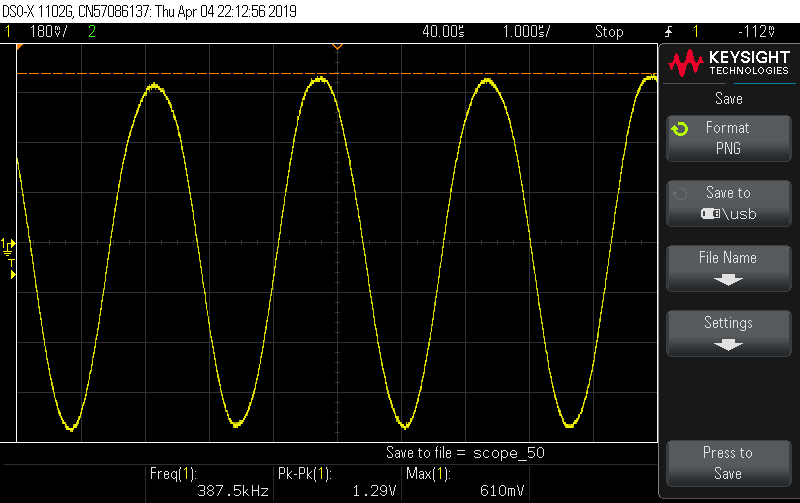
\includegraphics[width=\textwidth]{fig/P-crit.png}
	\caption{ Error signal of the QUIPS C master lock at the critical P-gain (current). The signal shows large amplitude oscillations with a frequency of \qty{390}{\kilo\hertz}. \label{fig:Pcrit}}
\end{figure}

\index{Current lock I-gain}\marginlabel{Current lock I-gain} 
After setting the P-gain, try to minimize the residual frequency fluctuations tuning the I-gain. Use the in-lock error signal (y deviation) as a measure. A larger value of the I-gain is preferable as long as no oscillatory behaviour is observable (check the corresponding output or the error signal with the 'scope' module in time mode).

\index{Piezo lock}\marginlabel{Piezo lock} 
Set the piezo P-gain to zero and the I-gain to a small value, e.g. 10. Activate the drift compensation by going to 'stage 1'. The mean output at 'out2' should now remain at zero. The piezo control loop should not influence the laser linewidth. If there is an noticeable increase of frequency fluctuations measured by the in-lock error signal when activating this stage, try to reduce the I-gain or apply an additional low-pass filter at 'Pz Out1'.

\subsection{Fine tuning and examples}

\index{Offset beat}\marginlabel{Offset beat}
Fine tuning of the PI-parameters can be achieved by monitoring the beat signal with a spectrum analyser when the laser is locked. Make sure the master laser is locked properly before optimizing the parameters. Note, that this method does not yield a laser linewidth . The beat linewidth is however a good measure for the performance of the offset lock. For our offset locks, the performance is typically limited by the noise and bandwidth (\qty{250}{\kilo\hertz}) of the frequency to voltage converters. It should be possible to obtain a linewidth of the beat below \qty{150}{\kilo\hertz} (FWHM).
 
\begin{figure}[H]
	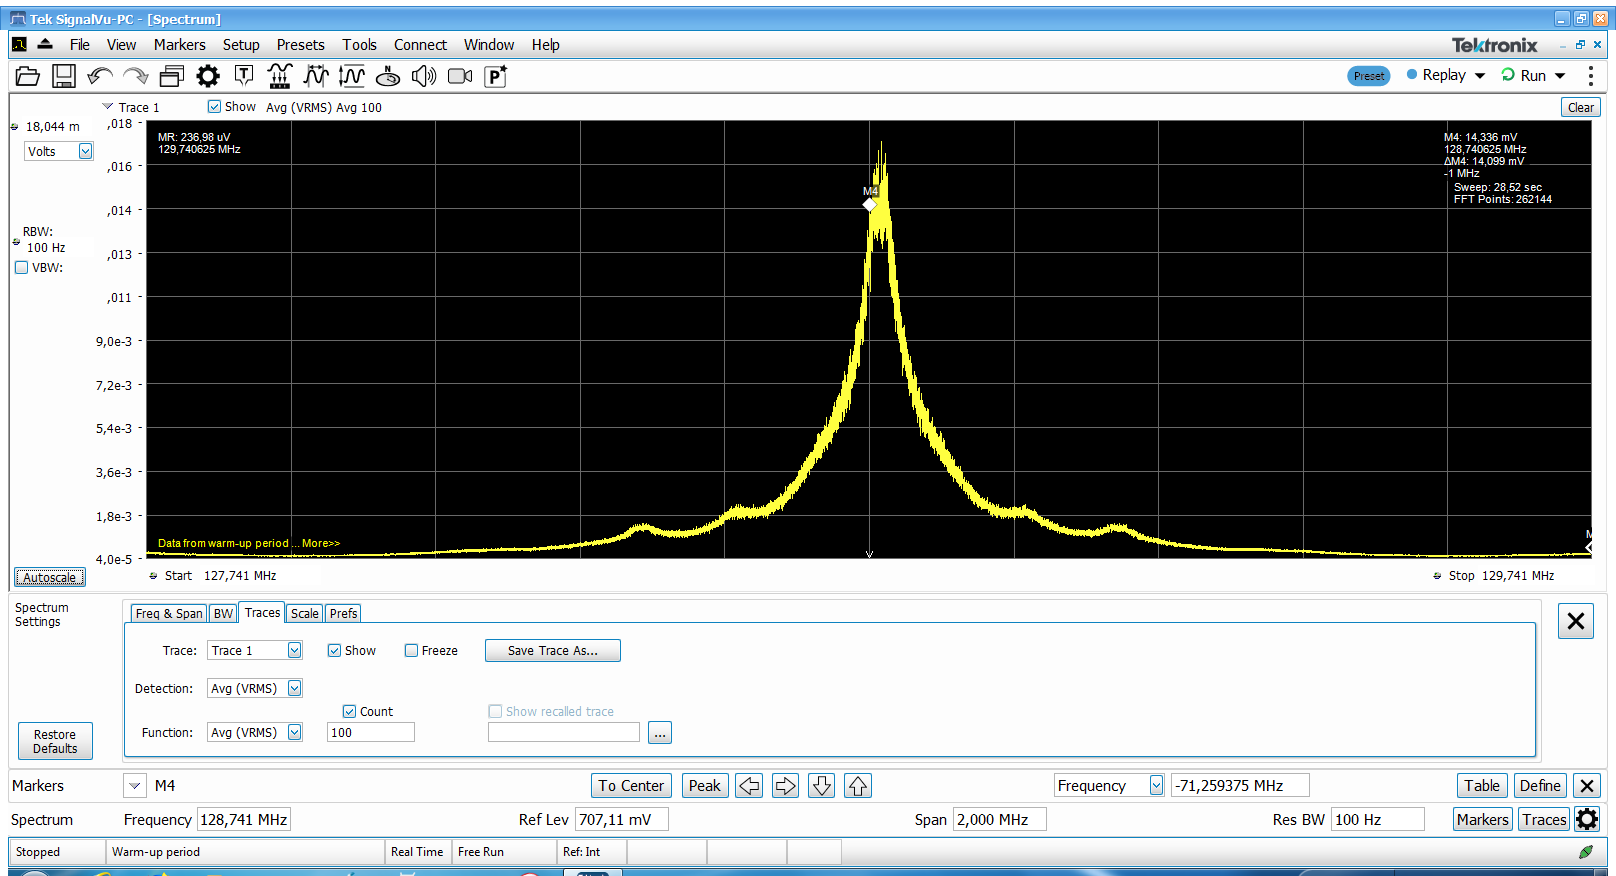
\includegraphics[width=\textwidth]{fig/offset_beat.png}
	\caption{Offset beat (QUIPS C master and TA seed laser) monitored with an RSA. Note, that the unconventional lineshape is caused by the influence of the large unfiltered DAC steps at the piezo in this case. \label{fig:offset_beat}}
\end{figure}

\index{Offset lock step response}\marginlabel{Offset lock step response}
Most offset locks allow for a fast change of the offset frequency setpoint. For our frequency to voltage converters, apply a voltage pulse with an appropriate offset to the reference voltage input (e.g. using an oscilloscope with signal generator). Make sure the amplitude does not exceed the voltage range of the fast actuator (usually approximately \qty{1}{\volt}) and both levels are in the linear region of the converter (e.g. centred at \qty{5}{\volt}). Watch the step response of the control loop at the 'Err Mon' output. Tune the PI parameters for minimal transient time or minimal overshoot depending on your application.

\begin{figure}[H]
	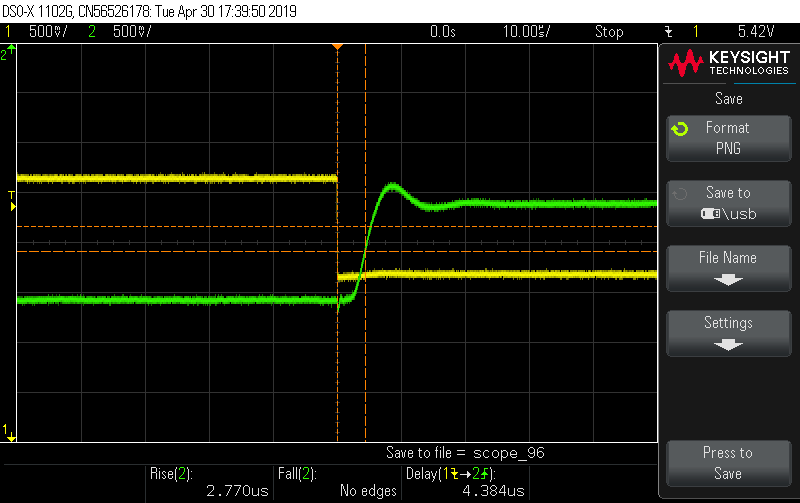
\includegraphics[width=\textwidth]{fig/step_response.png}
	\caption{Step response of an offset lock using a frequency to voltage converter (QUIPS C repump). \label{fig:offset_step}}
\end{figure}

\index{Master lock}\marginlabel{Master lock} 
Fine tuning of the PI parameters for the master laser lock is challenging since a real time measurement of the laser frequency noise is required. It is possible to use the beat with an independently stabilized laser with a sufficiently small linewidth for that purpose. The beat linewidth gives an upper bound to the linewidth of both lasers. In most cases, optimization with the in-loop error signal is sufficient. 

\begin{figure}[H]
	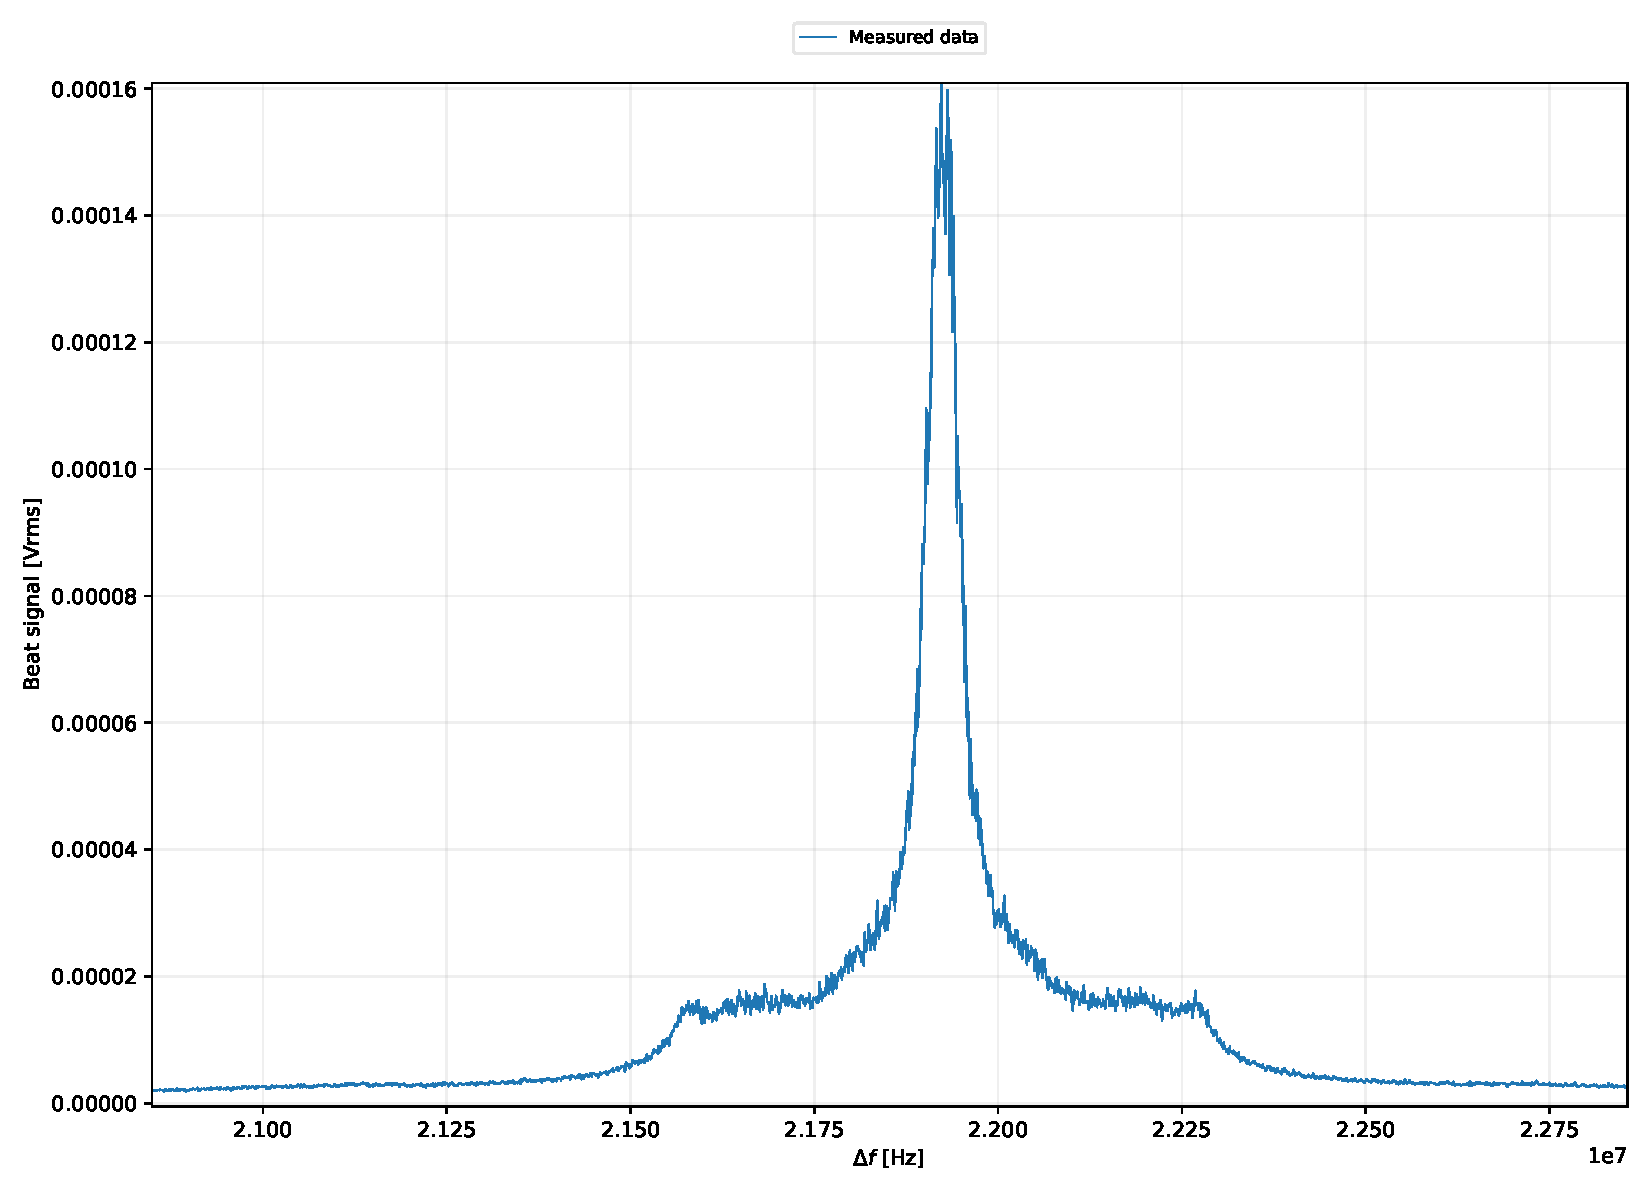
\includegraphics[width=\textwidth]{fig/master_beat.pdf}
	\caption{Beat of a master laser (QUIPS C) with an independently stabilized laser of a much smaller linewidth (Rydberg laser). \label{fig:master_beat}}
\end{figure}

\end{document}
